\chapter{CƠ SỞ LÝ THUYẾT VÀ CÔNG NGHỆ AGENTIC RAG}
\label{chap:theory}

Chương này trình bày nền tảng lý thuyết của đề tài theo trình tự từ tổng quát đến cụ thể: xử lý ngôn ngữ tự nhiên và mô hình ngôn ngữ lớn (Mục~\ref{sec:nlp_llm}); biểu diễn văn bản và truy xuất thông tin, gồm truy xuất thưa, truy xuất dày, truy xuất lai và xếp hạng lại (Mục~\ref{sec:ir}); kỹ thuật sinh văn bản tăng cường truy xuất (Mục~\ref{sec:rag}); tác tử AI và Agentic RAG (Mục~\ref{sec:agent}); phương pháp đánh giá hệ thống hỏi đáp dùng LLM (Mục~\ref{sec:eval_theory}); các công nghệ sử dụng (Mục~\ref{sec:tech}) và các nghiên cứu, sản phẩm liên quan (Mục~\ref{sec:related}). Phần RAG dựa trên bài báo gốc của Lewis và cộng sự~\cite{lewis2020rag} và bài tổng quan của Gao và cộng sự~\cite{gao2023ragsurvey}; phần Agent dựa trên mô hình ReAct~\cite{yao2023react} và các bài tổng quan về tác tử LLM~\cite{wang2024agentsurvey,singh2025agenticrag}.

% ==============================================================================
\section{Tổng quan về xử lý ngôn ngữ tự nhiên và mô hình ngôn ngữ lớn}
\label{sec:nlp_llm}

\subsection{Từ xử lý ngôn ngữ truyền thống đến mô hình ngôn ngữ lớn}
\label{sec:nlp_history}

Xử lý ngôn ngữ tự nhiên (Natural Language Processing -- NLP) là lĩnh vực nghiên cứu cách để máy tính hiểu, phân tích và sinh ra ngôn ngữ của con người. Các hệ thống NLP giai đoạn đầu dựa trên luật do chuyên gia viết tay và các mô hình thống kê trên đặc trưng rời rạc như túi từ (bag-of-words), n-gram hay TF-IDF. Cách biểu diễn này coi mỗi từ là một ký hiệu độc lập: hai từ ``kiếm'' và ``gươm'' không có quan hệ gì với nhau trong không gian đặc trưng, và văn bản được biểu diễn bằng vector rất thưa với số chiều bằng kích thước từ vựng.

Bước ngoặt đầu tiên là biểu diễn từ bằng vector dày (word embedding). Mô hình word2vec của Mikolov và cộng sự~\cite{mikolov2013word2vec} học vector vài trăm chiều cho mỗi từ bằng cách dự đoán từ từ ngữ cảnh xung quanh, nhờ đó các từ có nghĩa gần nhau nằm gần nhau trong không gian vector. Tuy vậy mỗi từ chỉ có một vector cố định, không phân biệt được nghĩa theo ngữ cảnh.

Năm 2017, kiến trúc Transformer~\cite{vaswani2017attention} thay thế mạng hồi quy bằng cơ chế tự chú ý (self-attention), cho phép mỗi từ ``nhìn'' toàn bộ câu cùng lúc và huấn luyện song song trên GPU. Trên nền Transformer, BERT~\cite{devlin2019bert} tiền huấn luyện bộ mã hóa hai chiều bằng nhiệm vụ đoán từ bị che, tạo ra biểu diễn phụ thuộc ngữ cảnh và trở thành nền của phần lớn mô hình hiểu ngôn ngữ, trong đó có các mô hình embedding câu dùng cho truy xuất (Mục~\ref{sec:dense}). Ở nhánh sinh văn bản, các mô hình chỉ gồm bộ giải mã được huấn luyện để dự đoán token tiếp theo trên lượng văn bản rất lớn. GPT-3~\cite{brown2020gpt3} với 175 tỷ tham số cho thấy mô hình đủ lớn có thể làm nhiều nhiệm vụ chỉ từ vài ví dụ trong prompt (few-shot) mà không cần huấn luyện lại. Sau đó, việc tinh chỉnh theo chỉ dẫn kết hợp học tăng cường từ phản hồi của con người~\cite{ouyang2022instructgpt} giúp mô hình làm theo yêu cầu tốt hơn, mở đường cho các trợ lý hội thoại hiện nay. Các mô hình gần đây còn hỗ trợ gọi công cụ (tool calling): mô hình trả về lời gọi hàm có tham số dạng JSON thay vì văn bản, là nền tảng để xây dựng tác tử (Mục~\ref{sec:agent}). Bảng~\ref{tab:nlp_milestones} tóm tắt các mốc chính liên quan đến đề tài.

\begin{table}[H]
    \centering
    \caption{Một số mốc phát triển của mô hình ngôn ngữ liên quan đến đề tài}
    \label{tab:nlp_milestones}
    \small
    \begin{tabularx}{\textwidth}{|c|>{\raggedright\arraybackslash}p{4.4cm}|>{\raggedright\arraybackslash}X|}
        \toprule
        \textbf{Năm} & \textbf{Mốc phát triển} & \textbf{Ý nghĩa đối với đề tài} \\
        \midrule
        2009 & BM25~\cite{robertson2009bm25}, RRF~\cite{cormack2009rrf} & Hàm xếp hạng từ khóa và cách hợp nhất nhiều danh sách xếp hạng, dùng trong truy xuất lai \\ \hline
        2013 & word2vec~\cite{mikolov2013word2vec} & Biểu diễn từ bằng vector dày, đặt nền cho embedding \\ \hline
        2017 & Transformer~\cite{vaswani2017attention} & Cơ chế self-attention, kiến trúc nền của mọi mô hình trong hệ thống \\ \hline
        2019 & BERT~\cite{devlin2019bert}, Sentence-BERT~\cite{reimers2019sbert} & Biểu diễn theo ngữ cảnh; embedding câu so khớp bằng cosine \\ \hline
        2020 & DPR~\cite{karpukhin2020dpr}, RAG~\cite{lewis2020rag}, GPT-3~\cite{brown2020gpt3} & Truy xuất dày cho hỏi đáp; kết hợp truy xuất với sinh; học ít mẫu trong prompt \\ \hline
        2022 & InstructGPT~\cite{ouyang2022instructgpt}, CoT~\cite{wei2022cot} & Mô hình làm theo chỉ dẫn; suy luận từng bước \\ \hline
        2023 & ReAct~\cite{yao2023react}, Toolformer~\cite{schick2023toolformer} & Mô hình xen kẽ suy luận với gọi công cụ \\ \hline
        2024 & Multilingual E5~\cite{wang2024me5}, Self-RAG~\cite{asai2024selfrag} & Embedding đa ngôn ngữ; mô hình tự quyết định khi nào truy xuất và tự phê bình \\ \hline
        2025 & Tổng quan Agentic RAG~\cite{singh2025agenticrag} & Hệ thống hóa các kiến trúc RAG do tác tử điều khiển \\
        \bottomrule
    \end{tabularx}
\end{table}

\subsection{Kiến trúc Transformer và cơ chế attention}
\label{sec:transformer}

Transformer gồm các khối chồng lên nhau, mỗi khối có một lớp tự chú ý nhiều đầu (multi-head self-attention) và một mạng truyền thẳng, kèm kết nối tắt và chuẩn hóa lớp~\cite{vaswani2017attention}. Với dãy đầu vào đã được biểu diễn thành ma trận $X$, mỗi đầu chú ý tính ba ma trận truy vấn $Q = XW^Q$, khóa $K = XW^K$ và giá trị $V = XW^V$, rồi tính đầu ra theo công thức scaled dot-product attention:
\begin{equation}
    \mathrm{Attention}(Q, K, V) = \mathrm{softmax}\!\left(\frac{QK^{\top}}{\sqrt{d_k}}\right) V,
    \label{eq:attention}
\end{equation}
trong đó $d_k$ là số chiều của vector khóa; phép chia cho $\sqrt{d_k}$ giữ cho tích vô hướng không quá lớn khiến softmax bão hòa. Mỗi hàng của ma trận softmax là phân phối trọng số cho biết một token cần ``chú ý'' bao nhiêu tới từng token khác. Nhiều đầu chú ý chạy song song cho phép mô hình học nhiều kiểu quan hệ cùng lúc (cú pháp, đồng tham chiếu, quan hệ ngữ nghĩa). Vì attention không có khái niệm thứ tự, Transformer cộng thêm mã hóa vị trí vào biểu diễn đầu vào.

Có hai cách dùng Transformer quan trọng với đề tài. Bộ mã hóa hai chiều (encoder, kiểu BERT) đọc cả câu và sinh vector biểu diễn, được dùng cho mô hình embedding E5 và bộ xếp hạng lại cross-encoder. Bộ giải mã một chiều (decoder, kiểu GPT) sinh token lần lượt từ trái sang phải với mặt nạ nhân quả, được dùng cho LLM sinh câu trả lời và điều khiển Agent.

\subsection{Hạn chế của mô hình ngôn ngữ lớn}
\label{sec:llm_limits}

Mặc dù rất mạnh, LLM có một số hạn chế ảnh hưởng trực tiếp đến bài toán hỏi đáp về một trò chơi cụ thể:
\begin{itemize}
    \item \textbf{Kiến thức tĩnh.} Tri thức của mô hình bị ``đóng băng'' tại thời điểm thu thập dữ liệu huấn luyện; các bản vá cân bằng vũ khí hay nội dung mới của bản mở rộng có thể không có trong tham số.
    \item \textbf{Ảo giác (hallucination).} Mô hình có thể sinh nội dung trôi chảy nhưng sai hoặc không có căn cứ~\cite{ji2023hallucination}. Với Elden Ring, lỗi điển hình là bịa vị trí vật phẩm, nhầm yêu cầu chỉ số vũ khí hoặc ghép nhầm hai nhân vật có tên gần giống.
    \item \textbf{Không trích dẫn được nguồn.} Tri thức nằm phân tán trong hàng tỷ tham số nên mô hình không chỉ ra được câu trả lời dựa trên tài liệu nào, khiến người dùng khó kiểm chứng.
    \item \textbf{Giới hạn ngữ cảnh.} Dù cửa sổ ngữ cảnh ngày càng dài, mô hình không dùng đều mọi vị trí: thông tin nằm giữa ngữ cảnh dài dễ bị bỏ qua hơn thông tin ở đầu hoặc cuối~\cite{liu2024lost}. Vì vậy đưa ít đoạn bằng chứng nhưng đúng trọng tâm thường tốt hơn đưa thật nhiều.
    \item \textbf{Tính toán kém tin cậy.} Các phép cộng trừ nhiều bước, như phân bổ tám chỉ số sao cho tổng đúng bằng level cộng 79, dễ sai khi mô hình ``tính nhẩm'' trong văn bản.
\end{itemize}
Các mục tiếp theo trình bày những kỹ thuật được dùng để khắc phục từng hạn chế: truy xuất để bổ sung tri thức có nguồn, kiểm tra trích dẫn để chống bịa, chọn lọc bằng chứng để tiết kiệm ngữ cảnh, và giao phép tính cho trình thông dịch.

\subsection{Kỹ thuật prompt và đầu ra có cấu trúc}
\label{sec:prompting}

Prompt là văn bản đầu vào điều khiển hành vi của LLM. Trong ứng dụng hội thoại, prompt thường chia thành thông điệp hệ thống (system prompt) mô tả vai trò và quy tắc, thông điệp người dùng chứa câu hỏi và dữ liệu, và các thông điệp trợ lý trước đó. Một số kỹ thuật được hệ thống sử dụng:
\begin{itemize}
    \item \textbf{Tách chỉ dẫn và dữ liệu.} Quy tắc nằm ở system prompt; đoạn bằng chứng, lịch sử và kết quả công cụ được đóng gói trong JSON ở thông điệp người dùng và được khai báo rõ là ``dữ liệu không tin cậy'', giảm nguy cơ văn bản trong tài liệu ghi đè chỉ dẫn (prompt injection).
    \item \textbf{Đầu ra có cấu trúc.} Yêu cầu mô hình trả về một đối tượng JSON theo lược đồ cố định (câu trả lời, danh sách bằng chứng, cờ thiếu thông tin) giúp máy chủ kiểm tra tự động từng trường.
    \item \textbf{Suy luận từng bước.} Chain-of-thought~\cite{wei2022cot} khuyến khích mô hình nêu các bước trung gian trước khi kết luận, cải thiện chất lượng với câu hỏi nhiều bước. Một số API, trong đó có DeepSeek, cung cấp ``chế độ suy nghĩ'' (thinking mode) sinh phần suy luận riêng trước câu trả lời; chế độ này tốn thêm token và thời gian nên hệ thống chỉ bật khi Agent đánh giá câu hỏi thật sự cần cân nhắc.
    \item \textbf{Gọi công cụ gốc (native tool calling).} Ứng dụng khai báo danh sách công cụ kèm lược đồ JSON Schema của tham số; mô hình trả về lời gọi công cụ thay vì văn bản; ứng dụng chạy công cụ và gửi kết quả lại cho mô hình ở lượt sau.
\end{itemize}

% ==============================================================================
\section{Biểu diễn văn bản và truy xuất thông tin}
\label{sec:ir}

Truy xuất thông tin (Information Retrieval) là bài toán tìm trong một tập lớn các tài liệu những tài liệu liên quan nhất tới một truy vấn. Trong RAG, chất lượng truy xuất quyết định trần chất lượng câu trả lời: nếu đoạn chứa đáp án không được tìm thấy, bước sinh dù tốt đến đâu cũng không thể trả lời đúng mà không bịa.

\subsection{Truy xuất thưa và hàm xếp hạng BM25}
\label{sec:bm25}

Truy xuất thưa (sparse retrieval) biểu diễn truy vấn và tài liệu bằng vector có số chiều bằng kích thước từ vựng, phần lớn bằng 0, và chấm điểm dựa trên các từ trùng nhau. Trọng số TF-IDF kết hợp tần suất của từ trong tài liệu (term frequency) với độ hiếm của từ trong toàn bộ tập tài liệu (inverse document frequency). BM25 là hàm xếp hạng phát triển từ mô hình xác suất về độ liên quan~\cite{robertson2009bm25}, bổ sung hai cải tiến: điểm tăng chậm dần khi một từ lặp lại nhiều lần (bão hòa tần suất), và tài liệu dài bị chuẩn hóa để không được lợi chỉ vì chứa nhiều từ. Điểm của tài liệu $d$ với truy vấn $q$ gồm các từ $t$ là
\begin{equation}
    \mathrm{BM25}(q, d) = \sum_{t \in q} \mathrm{IDF}(t)\cdot
    \frac{f(t, d)\,(k_1 + 1)}{f(t, d) + k_1\left(1 - b + b\,\dfrac{|d|}{\mathrm{avgdl}}\right)},
    \label{eq:bm25}
\end{equation}
với $f(t,d)$ là số lần từ $t$ xuất hiện trong $d$, $|d|$ là độ dài tài liệu, $\mathrm{avgdl}$ là độ dài trung bình, $k_1$ điều khiển mức bão hòa (thường 1,2--2,0) và $b$ điều khiển mức chuẩn hóa độ dài (thường 0,75). Thành phần IDF thường được tính bằng
\begin{equation}
    \mathrm{IDF}(t) = \ln\!\left(1 + \frac{N - n(t) + 0{,}5}{n(t) + 0{,}5}\right),
    \label{eq:idf}
\end{equation}
trong đó $N$ là tổng số tài liệu và $n(t)$ là số tài liệu chứa $t$.

BM25 có ưu điểm là nhanh, không cần huấn luyện và đặc biệt mạnh với tên riêng hiếm. Đây là điểm quan trọng với Elden Ring, nơi rất nhiều câu hỏi xoay quanh tên vật phẩm như ``Moonveil'' hay ``Rivers of Blood''. Nhược điểm của BM25 là không hiểu từ đồng nghĩa, không hiểu câu diễn đạt khác từ, và hoàn toàn bất lực khi truy vấn khác ngôn ngữ với tài liệu.

\subsection{Truy xuất dày và mô hình multilingual-E5}
\label{sec:dense}

Truy xuất dày (dense retrieval) dùng mạng nơ-ron mã hóa truy vấn và đoạn văn thành vector dày vài trăm chiều trong cùng một không gian, sao cho cặp liên quan có vector gần nhau. DPR~\cite{karpukhin2020dpr} dùng hai bộ mã hóa BERT huấn luyện với các cặp câu hỏi -- đoạn văn, vượt BM25 đáng kể trên nhiều bộ hỏi đáp mở. Sentence-BERT~\cite{reimers2019sbert} cho thấy có thể huấn luyện BERT theo kiến trúc Siamese để sinh embedding câu so sánh được bằng cosine, nhanh hơn nhiều so với đưa từng cặp câu qua BERT. Độ tương đồng giữa vector truy vấn $\mathbf{q}$ và vector đoạn văn $\mathbf{d}$ thường đo bằng cosine:
\begin{equation}
    \cos(\mathbf{q}, \mathbf{d}) = \frac{\mathbf{q}\cdot\mathbf{d}}{\lVert\mathbf{q}\rVert\,\lVert\mathbf{d}\rVert}.
    \label{eq:cosine}
\end{equation}
Khi các vector đã được chuẩn hóa về độ dài 1, cosine trùng với tích vô hướng.

Họ mô hình E5~\cite{wang2022e5} được tiền huấn luyện bằng học tương phản (contrastive learning) trên lượng rất lớn cặp văn bản thu thập từ web với giám sát yếu, sau đó tinh chỉnh trên dữ liệu có nhãn. Bản đa ngôn ngữ multilingual-E5~\cite{wang2024me5} mở rộng sang khoảng một trăm ngôn ngữ, trong đó có tiếng Việt, với các kích cỡ small, base và large. Hệ thống dùng bản nhỏ nhất \code{multilingual-e5-small} với vector 384 chiều và giới hạn 512 token đầu vào. Mô hình yêu cầu thêm tiền tố \code{query:} trước truy vấn và \code{passage:} trước đoạn văn để phân biệt hai vai trò. Ưu điểm lớn nhất với đề tài là khả năng truy xuất xuyên ngôn ngữ: câu hỏi tiếng Việt vẫn có thể tìm được đoạn tiếng Anh cùng nghĩa, dù chất lượng tốt hơn khi truy vấn cũng bằng tiếng Anh. Kích cỡ nhỏ cho phép chạy suy luận trên CPU qua ONNX Runtime mà không cần GPU.

Để tìm nhanh láng giềng gần nhất trong hàng chục nghìn vector, cơ sở dữ liệu vector dùng chỉ mục tìm kiếm gần đúng. Phổ biến nhất là đồ thị HNSW~\cite{malkov2020hnsw}, tổ chức các vector thành nhiều tầng đồ thị ``thế giới nhỏ'' để mỗi truy vấn chỉ cần duyệt một phần nhỏ của tập dữ liệu, đạt độ phức tạp gần logarit với độ chính xác rất cao.

\subsection{Truy xuất lai và hợp nhất thứ hạng Reciprocal Rank Fusion}
\label{sec:hybrid}

Truy xuất thưa và truy xuất dày có điểm mạnh bổ sung cho nhau: BM25 bắt chính xác tên riêng hiếm, còn embedding bắt được ý nghĩa khi cách diễn đạt khác nhau hoặc khác ngôn ngữ. Truy xuất lai (hybrid search) chạy song song cả hai rồi hợp nhất hai danh sách kết quả. Khó khăn là điểm số của hai phương pháp ở thang đo khác nhau (điểm BM25 không giới hạn trên, cosine nằm trong $[-1, 1]$) nên không cộng trực tiếp được.

Reciprocal Rank Fusion (RRF)~\cite{cormack2009rrf} giải quyết vấn đề này bằng cách chỉ dùng thứ hạng, bỏ qua điểm số. Với tập các danh sách xếp hạng $R$, điểm hợp nhất của tài liệu $d$ là
\begin{equation}
    \mathrm{RRF}(d) = \sum_{r \in R} \frac{1}{k + \mathrm{rank}_r(d)},
    \label{eq:rrf}
\end{equation}
trong đó $\mathrm{rank}_r(d)$ là vị trí của $d$ trong danh sách $r$ (tính từ 1) và $k$ là hằng số làm mượt; bài báo gốc dùng $k = 60$. Tài liệu đứng đầu ở nhiều danh sách được cộng điểm nhiều lần nên được đẩy lên trên, trong khi một danh sách đơn lẻ xếp sai không làm hỏng toàn bộ kết quả. Cormack và cộng sự cho thấy phương pháp đơn giản này cho kết quả tốt hơn phương pháp Condorcet và các phương pháp học xếp hạng riêng lẻ trong thử nghiệm của họ~\cite{cormack2009rrf}. RRF không cần huấn luyện và không cần chuẩn hóa điểm, nên phù hợp với hệ thống nhỏ.

\subsection{Xếp hạng lại bằng cross-encoder}
\label{sec:rerank}

Bộ mã hóa trong truy xuất dày (bi-encoder) mã hóa truy vấn và đoạn văn độc lập nên có thể tính trước vector của toàn bộ corpus, nhưng vì thế không mô hình hóa được tương tác chi tiết giữa từng từ của truy vấn với từng từ của đoạn văn. Cross-encoder ghép truy vấn và đoạn văn thành một chuỗi duy nhất đưa qua Transformer và xuất ra một điểm liên quan, nhờ attention giữa hai phần nên chính xác hơn nhiều. Nogueira và Cho~\cite{nogueira2019rerank} là một trong những công trình đầu tiên dùng BERT làm cross-encoder xếp hạng lại đoạn văn trên tập MS MARCO và đạt kết quả vượt trội so với các phương pháp trước đó. Đổi lại, cross-encoder phải chạy lại cho mỗi cặp nên chỉ dùng được cho vài chục ứng viên đứng đầu, theo mô hình hai giai đoạn: truy xuất nhanh lấy ứng viên, rồi xếp hạng lại chính xác.

Để chạy được trên CPU, có thể dùng cross-encoder nhỏ được chưng cất (distill) từ mô hình lớn. MiniLM~\cite{wang2020minilm} là kỹ thuật chưng cất cơ chế self-attention của mô hình thầy sang mô hình trò ít lớp và ít chiều hơn mà vẫn giữ phần lớn chất lượng. Hệ thống sử dụng một cross-encoder MiniLM 12 lớp đã được tinh chỉnh cho xếp hạng đoạn văn, chạy cục bộ qua ONNX.

\subsection{Cơ sở dữ liệu vector}
\label{sec:vectordb}

Cơ sở dữ liệu vector lưu vector kèm dữ liệu mô tả (payload) và hỗ trợ tìm láng giềng gần nhất có lọc theo payload. Hệ thống dùng Qdrant với các khái niệm chính sau:
\begin{itemize}
    \item \textbf{Collection}: tập các điểm (point) cùng cấu hình vector, tương tự một bảng.
    \item \textbf{Named vectors}: mỗi điểm có thể có nhiều vector đặt tên, ví dụ một vector dày \code{dense} (384 chiều, khoảng cách cosine) và một vector thưa \code{bm25} (chỉ lưu các chiều khác 0, Qdrant tự áp dụng IDF).
    \item \textbf{Payload}: dữ liệu JSON đi kèm mỗi điểm (tiêu đề, mục, URL, ngôn ngữ, phạm vi trò chơi\ldots), có thể đánh chỉ mục để lọc.
    \item \textbf{Prefetch và fusion}: Query API cho phép chạy nhiều truy vấn con (ví dụ một truy vấn dày và một truy vấn thưa) rồi hợp nhất kết quả bằng RRF ngay trong một lần gọi phía máy chủ.
\end{itemize}

\subsection{Chỉ số đánh giá truy xuất}
\label{sec:ir_metrics}

Cho mỗi câu hỏi $q$ trong tập đánh giá $Q$, gọi $G_q$ là tập tài liệu đúng (gold) và $T_q^{(k)}$ là $k$ tài liệu đứng đầu do hệ thống trả về. Các chỉ số dùng trong báo cáo được định nghĩa như sau:
\begin{equation}
    \mathrm{Recall@}k = \frac{1}{|Q|}\sum_{q \in Q} \frac{|G_q \cap T_q^{(k)}|}{|G_q|},
    \qquad
    \mathrm{Precision@}k = \frac{1}{|Q|}\sum_{q \in Q} \frac{|G_q \cap T_q^{(k)}|}{k},
    \label{eq:recall}
\end{equation}
\begin{equation}
    \mathrm{Hit@}k = \frac{1}{|Q|}\sum_{q \in Q} \mathbb{1}\!\left[G_q \cap T_q^{(k)} \neq \emptyset\right],
    \qquad
    \mathrm{MRR@}k = \frac{1}{|Q|}\sum_{q \in Q} \frac{1}{\mathrm{rank}_q},
    \label{eq:mrr}
\end{equation}
trong đó $\mathrm{rank}_q$ là vị trí của tài liệu đúng đầu tiên trong $k$ kết quả đầu (nếu không có thì $1/\mathrm{rank}_q = 0$). Recall@$k$ đo mức độ bao phủ, Hit@$k$ đo tỉ lệ câu có ít nhất một nguồn đúng, còn MRR@$k$ thưởng cho việc đặt nguồn đúng ở vị trí cao. Khi mỗi câu chỉ có một đến hai tài liệu đúng, Precision@5 có trần thực tế khoảng 0,2--0,4 nên chỉ dùng để so sánh tương đối giữa các cấu hình.

% ==============================================================================
\section{Retrieval-Augmented Generation}
\label{sec:rag}

\subsection{Định nghĩa và pipeline chuẩn}
\label{sec:rag_def}

Retrieval-Augmented Generation (RAG) là kỹ thuật kết hợp một bộ truy xuất với một mô hình sinh: trước khi sinh câu trả lời, hệ thống tìm các đoạn tài liệu liên quan và đưa chúng vào ngữ cảnh của mô hình. Lewis và cộng sự~\cite{lewis2020rag} đề xuất RAG năm 2020 với bộ truy xuất DPR và bộ sinh BART huấn luyện chung, gọi phần tri thức trong tham số là bộ nhớ tham số (parametric memory) và chỉ mục tài liệu là bộ nhớ phi tham số (non-parametric memory). Trong thực tế hiện nay, RAG thường được hiểu rộng hơn: dùng một LLM có sẵn, không huấn luyện lại, và chèn đoạn truy xuất vào prompt~\cite{gao2023ragsurvey}. Cách làm này có ba lợi ích: cập nhật tri thức chỉ bằng cách cập nhật chỉ mục, giảm ảo giác vì mô hình có căn cứ để dựa vào, và cho phép trích dẫn nguồn.

Pipeline RAG chuẩn gồm hai giai đoạn (Hình~\ref{fig:rag_pipeline}). Giai đoạn ngoại tuyến (offline) thu thập tài liệu, làm sạch, chia thành đoạn (chunk), mã hóa và lưu vào chỉ mục. Giai đoạn trực tuyến (online) nhận câu hỏi, truy xuất $k$ đoạn liên quan nhất, ghép chúng vào prompt (augment) và gọi LLM sinh câu trả lời.

\begin{figure}[H]
\centering
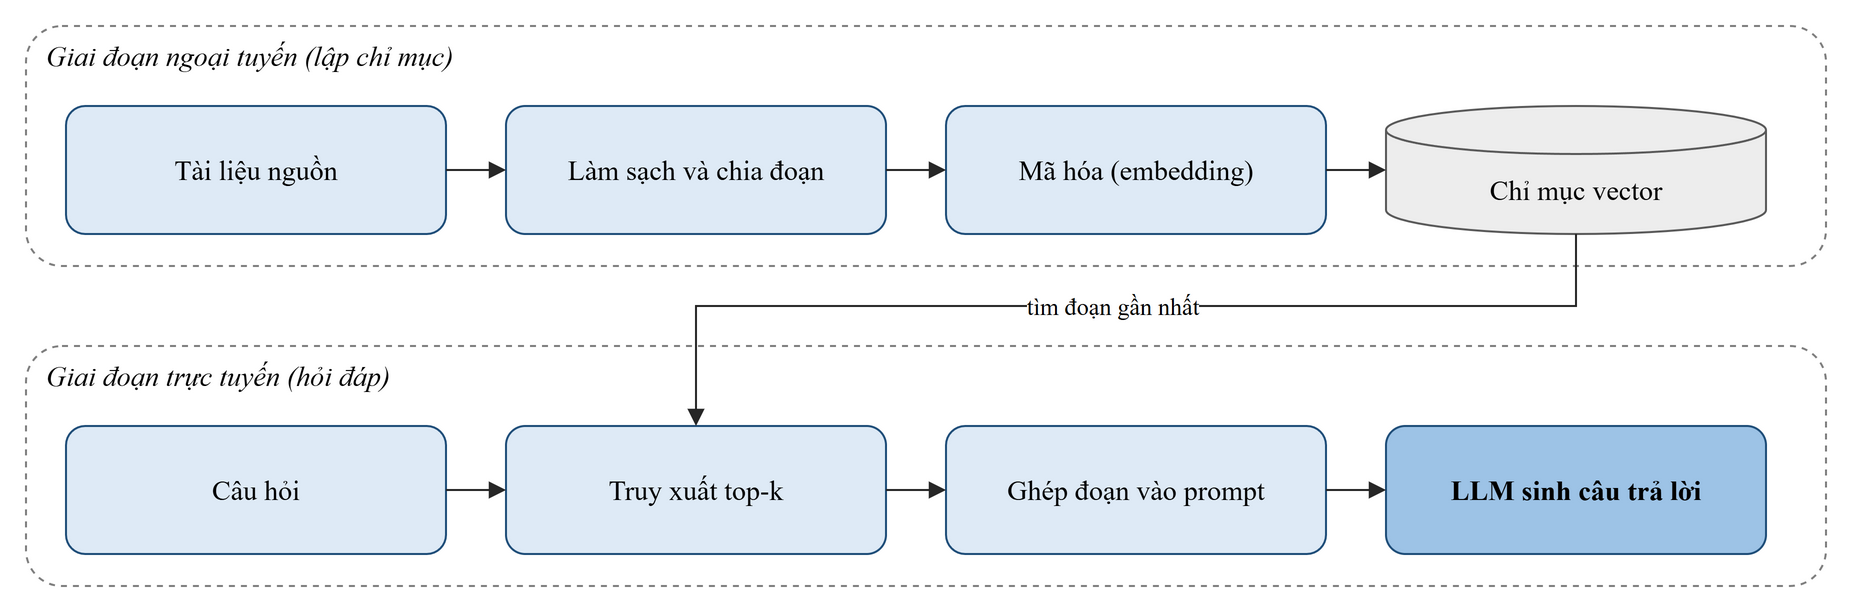
\includegraphics[width=\textwidth,height=0.62\textheight,keepaspectratio]{figures/rag_pipeline.png}
\caption{Pipeline RAG truyền thống gồm giai đoạn lập chỉ mục và giai đoạn hỏi đáp}
\label{fig:rag_pipeline}
\end{figure}

\subsection{Chia đoạn văn bản}
\label{sec:chunking}

Tài liệu thường quá dài để mã hóa thành một vector (E5 chỉ nhận 512 token) và quá dài để đưa nguyên vào prompt, nên phải chia thành các đoạn nhỏ. Cách chia ảnh hưởng mạnh tới chất lượng truy xuất. Chia theo độ dài cố định đơn giản nhưng dễ cắt ngang câu hoặc tách một ý khỏi tiêu đề của nó. Chia theo cấu trúc (theo tiêu đề mục của trang wiki) giữ được ranh giới tự nhiên của nội dung: mục ``Location'' của một vật phẩm nằm trọn trong một đoạn. Phần chồng lấn (overlap) giữa hai đoạn liên tiếp giảm rủi ro mất thông tin nằm ở ranh giới. Ngoài ra, gắn tiêu đề trang và tên mục vào mỗi đoạn giúp đoạn tự đủ nghĩa khi đứng một mình. Hệ thống chia theo mục với trần 450 token và chồng lấn 50 token (Mục~\ref{sec:kb_chunk}).

\subsection{Grounding và trích dẫn nguồn}
\label{sec:grounding}

Grounding (bám nguồn) là yêu cầu mọi khẳng định trong câu trả lời phải được hỗ trợ bởi bằng chứng đã truy xuất. Trích dẫn nguồn cho phép người dùng kiểm chứng và giúp phát hiện khi mô hình nói vượt quá bằng chứng. Gao và cộng sự~\cite{gao2023alce} xây dựng bộ đánh giá ALCE cho bài toán sinh văn bản kèm trích dẫn và cho thấy ngay cả các mô hình mạnh vẫn thường xuyên trích dẫn không đầy đủ hoặc trích dẫn đoạn không hỗ trợ khẳng định. Có hai mức kiểm tra trích dẫn:
\begin{itemize}
    \item \textbf{Kiểm tra hình thức} (có thể tự động hóa tất định): số trích dẫn trỏ tới bằng chứng có thật, đoạn trích dẫn có xuất hiện nguyên văn trong nguồn, không có đường dẫn do mô hình tự viết.
    \item \textbf{Kiểm tra ngữ nghĩa} (khó hơn): đoạn nguồn có thực sự hàm ý (entail) khẳng định hay không, thường cần một mô hình đánh giá hoặc con người.
\end{itemize}
Hệ thống \IB{} thực hiện đầy đủ kiểm tra hình thức ở máy chủ và để kiểm tra ngữ nghĩa cho bước đánh giá (Chương~\ref{chap:eval}).

\subsection{Hạn chế của RAG truyền thống}
\label{sec:rag_limits}

RAG truyền thống ``truy xuất một lần rồi sinh'' bộc lộ nhiều hạn chế với bài toán của đề tài:
\begin{itemize}
    \item \textbf{Truy vấn một lần, theo nguyên văn.} Câu tiếng Việt không dấu hoặc gõ sai tên riêng (``Malenia'' thành ``Melania'') được đưa thẳng vào bộ truy xuất, làm BM25 thất bại và embedding kém chính xác.
    \item \textbf{Không biết mình thiếu bằng chứng.} Nếu top-$k$ không chứa đáp án, hệ thống vẫn sinh câu trả lời từ những gì có, dễ dẫn tới bịa.
    \item \textbf{Không hỏi lại.} Với câu mơ hồ như ``hiệp sĩ đó ở Roundtable Hold'', hệ thống chọn đại một cách hiểu.
    \item \textbf{Không suy luận nhiều bước.} Câu hỏi nhiệm vụ cần nối thông tin từ nhiều trang, hoặc cần tìm thêm sau khi đọc kết quả đầu, vượt quá một lượt truy xuất.
    \item \textbf{Không tính toán.} Câu hỏi về phân bổ chỉ số cần số liệu của lớp nhân vật, yêu cầu của vũ khí và một phép tính có kiểm tra.
\end{itemize}
Các biến thể RAG nâng cao như viết lại truy vấn, tự đánh giá độ liên quan của tài liệu~\cite{yan2024crag} hay mô hình tự quyết định khi nào cần truy xuất~\cite{asai2024selfrag} giải quyết từng phần. Hướng tổng quát hơn là để một tác tử điều khiển toàn bộ quá trình, gọi là Agentic RAG.

% ==============================================================================
\section{Tác tử AI và Agentic RAG}
\label{sec:agent}

\subsection{Khái niệm tác tử AI}
\label{sec:agent_def}

Tác tử (agent) là một hệ thống tự cảm nhận môi trường, suy luận và hành động để đạt mục tiêu. Tác tử dựa trên LLM dùng mô hình ngôn ngữ làm ``bộ não'' điều khiển. Theo tổng quan của Wang và cộng sự~\cite{wang2024agentsurvey}, một tác tử LLM thường gồm bốn thành phần: hồ sơ (profile) xác định vai trò; bộ nhớ (memory) lưu thông tin từ các lượt trước; lập kế hoạch (planning) phân rã mục tiêu thành các bước; và hành động (action) thực thi qua công cụ. Khác với một lời gọi LLM đơn lẻ, tác tử hoạt động theo vòng lặp: quan sát kết quả hành động trước rồi quyết định hành động tiếp theo cho tới khi đạt mục tiêu hoặc hết ngân sách.

\subsection{Gọi công cụ}
\label{sec:tool_calling}

Gọi công cụ (tool calling hay function calling) cho phép LLM tương tác với thế giới bên ngoài. Toolformer~\cite{schick2023toolformer} cho thấy mô hình có thể tự học khi nào và cách nào gọi API như máy tính, công cụ tìm kiếm hay hệ thống hỏi đáp để cải thiện kết quả. Trong các API hiện đại, cơ chế này được hỗ trợ trực tiếp. Ứng dụng khai báo cho mỗi công cụ một tên, một mô tả ngắn và lược đồ JSON Schema của tham số. Ở mỗi lượt, mô hình có thể trả về văn bản hoặc một hay nhiều lời gọi công cụ. Ứng dụng kiểm tra tham số, chạy công cụ, rồi thêm kết quả vào hội thoại dưới dạng thông điệp công cụ (tool message) gắn với mã lời gọi. Vì lược đồ tham số được kiểm tra ở phía ứng dụng, lời gọi sai có thể bị từ chối kèm thông báo lỗi để mô hình tự sửa ở lượt sau.

\subsection{Mô hình suy luận ReAct}
\label{sec:react}

ReAct (Reasoning and Acting)~\cite{yao2023react} là mô hình để LLM xen kẽ giữa suy nghĩ và hành động. Ở mỗi bước, mô hình viết một suy nghĩ (thought) phân tích tình huống, chọn một hành động (action) như tìm kiếm, rồi nhận về quan sát (observation) là kết quả của hành động. Chu trình lặp lại cho tới khi mô hình đưa ra câu trả lời cuối (Hình~\ref{fig:react}). So với chỉ suy luận (chain-of-thought), ReAct cho phép mô hình lấy thêm thông tin thật thay vì dựa vào trí nhớ, giảm ảo giác; so với chỉ hành động, phần suy nghĩ giúp mô hình lập kế hoạch và xử lý ngoại lệ. Trên các bộ hỏi đáp nhiều bước như HotpotQA, ReAct cho kết quả bám sự kiện tốt hơn chain-of-thought thuần~\cite{yao2023react}.

\begin{figure}[H]
\centering
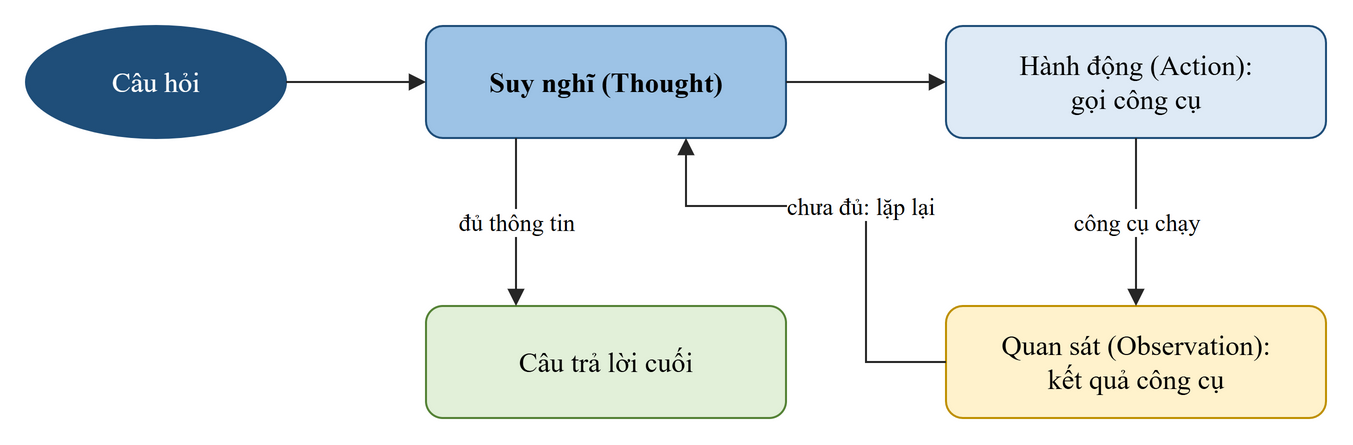
\includegraphics[width=0.85\textwidth,height=0.62\textheight,keepaspectratio]{figures/react_loop.png}
\caption{Vòng lặp suy nghĩ -- hành động -- quan sát của mô hình ReAct}
\label{fig:react}
\end{figure}

Một số công trình mở rộng vòng lặp này bằng khả năng tự phản tư. Self-RAG~\cite{asai2024selfrag} huấn luyện mô hình sinh các token đặc biệt để tự quyết định khi nào truy xuất và tự đánh giá đoạn truy xuất có liên quan, câu trả lời có được hỗ trợ hay không. Corrective RAG~\cite{yan2024crag} thêm một bộ đánh giá nhẹ chấm chất lượng tài liệu truy xuất; khi tài liệu kém, hệ thống chuyển sang tìm kiếm web và lọc lại nội dung.

\subsection{Agentic RAG}
\label{sec:agentic_rag}

Agentic RAG là kiến trúc trong đó một hoặc nhiều tác tử điều khiển quá trình truy xuất thay cho một pipeline cố định~\cite{singh2025agenticrag}. Thay vì luôn truy xuất một lần theo nguyên văn câu hỏi, tác tử có thể: viết lại và dịch truy vấn; chia câu hỏi phức tạp thành nhiều truy vấn con; tìm nhiều lần và đổi chiến lược khi kết quả chưa đủ; chọn giữa nhiều nguồn (kho nội bộ, web, cơ sở dữ liệu có cấu trúc); kiểm tra lại kết quả; dùng công cụ tính toán; và hỏi lại người dùng khi câu hỏi mơ hồ. Singh và cộng sự hệ thống hóa các mẫu hành vi tác tử thường gặp (phản tư, lập kế hoạch, dùng công cụ, phối hợp nhiều tác tử) và phân loại kiến trúc Agentic RAG, chẳng hạn một tác tử, nhiều tác tử hay phân cấp~\cite{singh2025agenticrag}. Bảng~\ref{tab:compare_paradigm} so sánh ba cách tiếp cận cho bài toán hỏi đáp của đề tài.

\begin{table}[H]
    \centering
    \caption{So sánh chatbot dựa trên luật, RAG truyền thống và Agentic RAG}
    \label{tab:compare_paradigm}
    \small
    \begin{tabularx}{\textwidth}{|>{\raggedright\arraybackslash}p{2.7cm}|>{\raggedright\arraybackslash}X|>{\raggedright\arraybackslash}X|>{\raggedright\arraybackslash}X|}
        \toprule
        \textbf{Tiêu chí} & \textbf{Chatbot dựa trên luật / FAQ} & \textbf{RAG truyền thống} & \textbf{Agentic RAG} \\
        \midrule
        Cách truy xuất & Khớp từ khóa hoặc mẫu câu viết tay & Một lần, theo nguyên văn câu hỏi & Nhiều lần, truy vấn do tác tử viết, có thể đổi nguồn \\ \hline
        Câu gõ sai, khác ngôn ngữ & Thất bại & Phụ thuộc embedding & Tác tử dịch, kiểm tên rồi tìm lại \\ \hline
        Câu mơ hồ & Trả lời theo mẫu gần nhất & Chọn đại một cách hiểu & Có thể hỏi lại người dùng \\ \hline
        Câu nhiều bước & Không hỗ trợ & Hạn chế trong top-$k$ & Tìm tiếp dựa trên kết quả trước \\ \hline
        Tính toán & Chỉ khi viết sẵn & Mô hình tính nhẩm & Gọi công cụ tính toán \\ \hline
        Trích dẫn nguồn & Có thể gắn sẵn & Có, tùy cách sinh & Có, tác tử chọn bằng chứng \\ \hline
        Chi phí, độ trễ & Rất thấp & Thấp (một lượt LLM) & Cao hơn (nhiều lượt LLM) \\
        \bottomrule
    \end{tabularx}
\end{table}

\subsection{Một tác tử và nhiều tác tử}
\label{sec:single_multi}

Hệ thống nhiều tác tử (multi-agent) chia công việc cho các tác tử chuyên trách, ví dụ một tác tử phân loại câu hỏi, một tác tử tìm kiếm, một tác tử đánh giá bằng chứng, rồi phối hợp qua một bộ điều phối. Cách này dễ chuyên môn hóa prompt cho từng vai và có thể chạy song song. Nhược điểm là mỗi tác tử chỉ thấy một phần ngữ cảnh, thông tin bị mất khi chuyển giữa các vai, số lượt gọi LLM và độ trễ tăng, và lỗi của tác tử trước lan sang tác tử sau. Hệ thống một tác tử dùng một vòng lặp duy nhất với đầy đủ ngữ cảnh: tác tử vừa hiểu câu hỏi, vừa tìm kiếm, vừa đánh giá bằng chứng. Với bài toán hỏi đáp có phạm vi rõ như của đề tài, một tác tử với bộ công cụ tốt thường đủ dùng, đơn giản hơn để gỡ lỗi và tiết kiệm hơn. Mục~\ref{sec:agent_role} trình bày lý do nhóm chọn kiến trúc một tác tử.

\subsection{Bộ nhớ cho tác tử}
\label{sec:memory}

Bộ nhớ giúp tác tử duy trì mạch hội thoại và cá nhân hóa câu trả lời~\cite{wang2024agentsurvey}. Có thể chia thành:
\begin{itemize}
    \item \textbf{Bộ nhớ ngắn hạn}: các lượt gần nhất của hội thoại hiện tại, được đưa thẳng vào prompt để tác tử hiểu các tham chiếu như ``con boss đó''.
    \item \textbf{Bộ nhớ dài hạn hay bộ nhớ ngữ nghĩa}: các mục nhớ được mã hóa thành vector và lưu trong cơ sở dữ liệu; khi có câu hỏi mới, hệ thống truy xuất các mục liên quan bằng độ tương đồng thay vì đưa toàn bộ lịch sử. MemGPT~\cite{packer2023memgpt} đề xuất quản lý bộ nhớ của LLM theo phân cấp giống hệ điều hành, chuyển thông tin giữa ngữ cảnh chính và bộ nhớ ngoài.
    \item \textbf{Trạng thái làm việc}: dữ kiện có cấu trúc của nhiệm vụ đang làm, ví dụ level, lớp nhân vật, vũ khí người chơi đã nêu.
\end{itemize}
Một nguyên tắc quan trọng là bộ nhớ chỉ cho biết người dùng đã nói gì, không phải nguồn tri thức về trò chơi; dữ kiện về game vẫn phải lấy từ tài liệu có trích dẫn.

% ==============================================================================
\section{Đánh giá hệ thống hỏi đáp dùng mô hình ngôn ngữ lớn}
\label{sec:eval_theory}

Đánh giá hệ thống RAG cần tách riêng chất lượng truy xuất và chất lượng câu trả lời~\cite{gao2023ragsurvey,es2024ragas}. Truy xuất được đo bằng các chỉ số ở Mục~\ref{sec:ir_metrics} trên tập câu hỏi có gắn nhãn nguồn đúng. Câu trả lời thường được đánh giá theo ba khía cạnh:
\begin{itemize}
    \item \textbf{Độ đúng (correctness)}: câu trả lời có khớp với đáp án tham chiếu về các ý chính hay không.
    \item \textbf{Độ bám nguồn (faithfulness hoặc groundedness)}: các khẳng định có được nguồn đã trích hỗ trợ hay không. RAGAS~\cite{es2024ragas} đề xuất đo faithfulness bằng cách tách câu trả lời thành các mệnh đề rồi dùng LLM kiểm tra từng mệnh đề có suy ra được từ ngữ cảnh.
    \item \textbf{Hành vi đúng}: với câu ngoài phạm vi phải từ chối, với câu thiếu dữ kiện phải hỏi lại hoặc nêu rõ các khả năng.
\end{itemize}

Chấm tay chính xác nhưng tốn công, nên nhiều nghiên cứu dùng LLM làm người chấm (LLM-as-a-judge). Zheng và cộng sự~\cite{zheng2023judge} cho thấy các LLM mạnh đạt mức đồng thuận với người chấm tương đương mức đồng thuận giữa hai người, nhưng cũng chỉ ra các thiên lệch như ưu tiên câu trả lời dài, ưu tiên vị trí và ưu tiên câu do chính mô hình đó sinh. Vì vậy cần một rubric rõ ràng, đối chiếu một phần với người chấm và ghi rõ người chấm khi báo cáo.

Bên cạnh chất lượng, hệ thống dùng LLM cần được đánh giá về vận hành: độ trễ đầu cuối theo phân vị p50 và p95, số lượt gọi mô hình mỗi câu hỏi, số token vào và ra, và chi phí ước tính.

% ==============================================================================
\section{Các công nghệ sử dụng}
\label{sec:tech}

Bảng~\ref{tab:techstack} liệt kê các công nghệ chính của hệ thống theo từng tầng. Nhóm chọn công nghệ theo nguyên tắc tối giản, có thể chạy trên một máy chủ 4 vCPU và 8 GB RAM, và ghim cứng phiên bản để mọi thành viên có môi trường giống nhau.

\begin{table}[H]
    \centering
    \caption{Công nghệ sử dụng trong hệ thống \IB{}}
    \label{tab:techstack}
    \small
    \begin{tabularx}{\textwidth}{|>{\raggedright\arraybackslash}p{3.2cm}|>{\raggedright\arraybackslash}p{4.3cm}|>{\raggedright\arraybackslash}X|}
        \toprule
        \textbf{Tầng} & \textbf{Công nghệ (phiên bản)} & \textbf{Vai trò trong hệ thống} \\
        \midrule
        Mô hình ngôn ngữ & DeepSeek \code{deepseek-flash} (API) & Điều khiển vòng lặp Agent bằng native tool calling và sinh câu trả lời JSON \\ \hline
        Điều phối LLM & LangChain: langchain-core 1.7.1, langchain-deepseek 1.1.1 & Lớp trừu tượng gọi mô hình, prompt template, \code{bind\_tools} \\ \hline
        Đồ thị xử lý & LangGraph 1.2.20 & \code{StateGraph} cho bước chuẩn bị (scope -- memory -- agent -- context -- prompt) và bước sinh -- kiểm -- sửa \\ \hline
        Embedding & multilingual-e5-small (ONNX, 384 chiều), fastembed 0.9.0 & Mã hóa đoạn văn và truy vấn, chạy trên CPU \\ \hline
        Truy xuất thưa & Qdrant/bm25 & Vector thưa BM25, IDF tính ở Qdrant \\ \hline
        Xếp hạng lại & ms-marco-MiniLM-L-12-v2 (ONNX) & Cross-encoder chạy cục bộ, xếp hạng lại ứng viên sau RRF \\ \hline
        Cơ sở dữ liệu vector & Qdrant 1.19 & Lưu corpus (dense + sparse) và bộ nhớ ngữ nghĩa \\ \hline
        Cơ sở dữ liệu quan hệ & PostgreSQL 18, SQLAlchemy, Alembic & Tài liệu, đoạn, hội thoại, trace, người dùng \\ \hline
        Bộ nhớ đệm & Redis 8 & Giới hạn tần suất và hạn mức hằng ngày \\ \hline
        Tìm kiếm web & Tavily Search + Extract & Bổ sung bằng chứng khi kho nội bộ chưa đủ \\ \hline
        Backend & Python 3.11, FastAPI 0.143, Uvicorn & API JSON và SSE \\ \hline
        Giao diện web & React 19, Vite 8, Tailwind CSS 4 & Khung chat, nguồn trích dẫn, trang quản trị \\ \hline
        Discord bot & discord.js 14, Node.js 24 & Lệnh \code{/ask}, trả lời khi được nhắc tên \\ \hline
        Triển khai & Docker Compose, Caddy 2, GitHub Actions & Đóng gói dịch vụ, HTTPS tự động, CI \\
        \bottomrule
    \end{tabularx}
\end{table}

\textbf{DeepSeek.} DeepSeek là họ mô hình ngôn ngữ lớn có API tương thích định dạng OpenAI. Báo cáo kỹ thuật DeepSeek-V3~\cite{deepseek2024v3} mô tả kiến trúc Mixture-of-Experts của dòng mô hình này, trong đó mỗi token chỉ kích hoạt một phần tham số, giúp chi phí suy luận thấp. Hệ thống dùng mô hình \code{deepseek-flash} qua API với hai tính năng chính: gọi công cụ gốc cho vòng lặp Agent và chế độ trả về JSON cho bước sinh câu trả lời. Chế độ suy nghĩ được tắt ở các lượt Agent và chỉ được phép bật ở bước viết với những câu Agent đánh dấu cần cân nhắc.

\textbf{LangChain và LangGraph.} LangChain cung cấp lớp trừu tượng thống nhất cho mô hình, prompt và bộ truy xuất; hệ thống dùng \code{ChatDeepSeek}, \code{ChatPromptTemplate} và giao diện \code{BaseRetriever}. LangGraph biểu diễn luồng xử lý thành đồ thị có trạng thái (\code{StateGraph}): mỗi nút là một hàm nhận và cập nhật trạng thái, các cạnh (kể cả cạnh có điều kiện) quyết định nút tiếp theo. Cách tổ chức này giúp tách từng bước, ghi thời gian từng nút vào trace và dễ kiểm thử.

\textbf{Qdrant.} Qdrant là cơ sở dữ liệu vector mã nguồn mở viết bằng Rust, hỗ trợ đồng thời vector dày và vector thưa trên cùng một điểm, lọc theo payload và hợp nhất RRF phía máy chủ qua Query API. Nhờ đó toàn bộ truy xuất lai chỉ cần một lần gọi.

\textbf{FastAPI, React và discord.js.} FastAPI là framework web bất đồng bộ của Python, sinh tài liệu OpenAPI tự động từ lược đồ Pydantic. React kết hợp Vite và Tailwind CSS dùng cho giao diện web; luồng SSE được đọc bằng \code{fetch} và \code{ReadableStream}. Discord bot viết bằng discord.js và TypeScript, chạy trực tiếp trên Node.js 24.

\textbf{Docker Compose và Caddy.} Toàn bộ dịch vụ (PostgreSQL, Qdrant, Redis, API, Caddy, bot) được đóng gói bằng Docker Compose. Caddy làm reverse proxy, tự cấp chứng chỉ HTTPS, phục vụ web tĩnh và chuyển tiếp \code{/api} mà không đệm luồng SSE.

% ==============================================================================
\section{Các nghiên cứu và sản phẩm liên quan}
\label{sec:related}

\textbf{Wiki cộng đồng.} Các wiki như eldenring.wiki.gg hay Fextralife là nguồn tra cứu chính của người chơi. Chúng có nội dung chi tiết và được cập nhật thường xuyên, nhưng chỉ tìm kiếm theo từ khóa tiếng Anh, không tổng hợp thông tin từ nhiều trang và không trả lời trực tiếp một câu hỏi tự nhiên.

\textbf{Chatbot tổng quát.} Các trợ lý như ChatGPT trả lời bằng tiếng Việt trôi chảy, nhưng với chi tiết cụ thể của trò chơi thường sai lệch và không kèm nguồn kiểm chứng được, đúng với các hạn chế đã nêu ở Mục~\ref{sec:llm_limits}.

\textbf{Các hệ RAG và Agentic RAG trong nghiên cứu.} RAG gốc~\cite{lewis2020rag} và các biến thể như Self-RAG~\cite{asai2024selfrag}, Corrective RAG~\cite{yan2024crag} tập trung vào bộ dữ liệu hỏi đáp mở tiếng Anh như Wikipedia. Các bài tổng quan~\cite{gao2023ragsurvey,singh2025agenticrag} hệ thống hóa kỹ thuật nhưng không đi vào một miền cụ thể với câu hỏi song ngữ, gõ sai và yêu cầu tính toán.

Bảng~\ref{tab:related} tóm tắt các giải pháp và khoảng trống mà \IB{} hướng tới.

\begin{table}[H]
    \centering
    \caption{Tóm tắt giải pháp liên quan và khoảng trống mà \IB{} hướng tới}
    \label{tab:related}
    \small
    \begin{tabularx}{\textwidth}{|>{\raggedright\arraybackslash}p{3.3cm}|>{\raggedright\arraybackslash}X|>{\raggedright\arraybackslash}X|}
        \toprule
        \textbf{Giải pháp} & \textbf{Điểm mạnh} & \textbf{Hạn chế với bài toán} \\
        \midrule
        Wiki cộng đồng & Đầy đủ, cập nhật, có nguồn & Chỉ tiếng Anh, tìm theo từ khóa, không tổng hợp \\ \hline
        Chatbot tổng quát & Hội thoại tự nhiên, tiếng Việt tốt & Bịa chi tiết game, không có nguồn \\ \hline
        RAG truyền thống & Có căn cứ, có nguồn & Một lần truy xuất, yếu với câu gõ sai, mơ hồ, nhiều bước, cần tính toán \\ \hline
        Self-RAG, CRAG & Tự đánh giá truy xuất & Thiết kế cho hỏi đáp mở tiếng Anh, cần huấn luyện hoặc bộ đánh giá riêng \\ \hline
        \textbf{\IB{}} & Agent tự tìm, kiểm tên, tính toán, hỏi lại; trích dẫn kiểm nguyên văn; song ngữ Việt -- Anh; Web và Discord & Phụ thuộc chất lượng corpus và API LLM bên ngoài \\
        \bottomrule
    \end{tabularx}
\end{table}

% ==============================================================================
\section{Tóm tắt chương}
\label{sec:ch1_summary}

Chương này đã trình bày các nền tảng lý thuyết của đề tài. LLM dựa trên Transformer có khả năng ngôn ngữ mạnh nhưng có kiến thức tĩnh, dễ ảo giác và không trích dẫn được nguồn. Truy xuất lai kết hợp BM25 với embedding multilingual-E5, hợp nhất bằng RRF và xếp hạng lại bằng cross-encoder, giúp tìm bằng chứng tốt cho cả tên riêng lẫn câu hỏi khác ngôn ngữ. RAG đưa bằng chứng vào ngữ cảnh để sinh câu trả lời có căn cứ, còn Agentic RAG để một tác tử điều khiển quá trình tìm kiếm, kiểm tra, tính toán và hỏi lại theo vòng lặp ReAct. Chương~\ref{chap:design} áp dụng các nền tảng này vào phân tích và thiết kế hệ thống \IB{}.
